%%%%%%%%%%%%%%%%%%%%%%%%%%%%%%%%%%%%%%%%%%%%%%%%%%%%%%%%%%%%%%%%%%%%%%%%%%%%%%%%%%%%%%%%%%%%%%%%%%%%%%%%%%%%%%%%%%%%%%%%%%%%%%%%%%%%%%%%%%%%%%%%%%%%%%%%%%%%%%%%%%%
% Written By Michael Brodskiy
% Class: Modern Physics
% Professor: Q. Yan
%%%%%%%%%%%%%%%%%%%%%%%%%%%%%%%%%%%%%%%%%%%%%%%%%%%%%%%%%%%%%%%%%%%%%%%%%%%%%%%%%%%%%%%%%%%%%%%%%%%%%%%%%%%%%%%%%%%%%%%%%%%%%%%%%%%%%%%%%%%%%%%%%%%%%%%%%%%%%%%%%%%

\include{Includes.tex}

\title{Homework 6}
\date{March 29, 2023}
\author{Michael Brodskiy\\ \small Professor: Q. Yan}

\begin{document}

\maketitle

\newpage

\begin{enumerate}

    \section*{Permitted Wave Functions}

    \begin{enumerate}

      \item One reason why this function is not permitted is because it violates the normalization condition, $\displaystyle \int_{-\infty}^{\infty}|\psi(x)|^2\,dx=1$; more specifically, solving for the boundary conditions makes it violate this:

        $$A\cos(kx)=B\sin(kx)$$
        $$A\cos(0)=B\sin(0)$$
        $$A=0$$

        Differentiating to find $B$:

        $$0=Bk\cos(kx)$$
        $$B=0$$

        Because both constants are zero, the integral over the entire boundary does not equal 1.

      \item $\psi(x)=\dfrac{Ae^{-kx}}{x}$ can not be a solution because it is discontinuous; at the point $x=0$, the function has a discontinuity.

      \item $A\sin^{-1}(kx)$ can not be a solution because it is discontinuous. $\sin^{-1}$ is only valid for values in the range $\left(-\dfrac{\pi}{2}, \dfrac{\pi}{2}\right)$, and, thus, it must have a discontinuity somewhere in its domain, unless $k$ were to have the value of zero; in such a case, the function would violate the normalization condition, as it would be zero over its whole domain.

      \item $A\tan(kx)$ can not be a solution because it is discontinuous every $n\pi$ intervals.

    \end{enumerate}

    \section*{The Schr\"odinger Equation}

    For a particle with $\psi(x)=Cxe^{-bx}$, plugging into the Schr\"odinger equation would yield:

    $$\left( -\dfrac{\hbar^2}{2m} \right)(b^2Cxe^{-bx}-2bCe^{-bx})+U(x)(Cxe^{-bx})=E(Cxe^{-bx})$$
    $$E=\left( -\dfrac{\hbar^2}{2m} \right)\left(b^2-\frac{2b}{x}\right)+U(x)$$

    The $x$ terms balance and cancel out because $E$ is constant:

    $$E=-\dfrac{\hbar^2b^2}{2m}$$

    This makes $U(x)$ equal to the final term left when $E$ cancels out:

    $$U(x)=-\dfrac{b\hbar^2}{mx}$$

    \section*{Expectation Values}

    \begin{enumerate}

      \item In ground state ($n=1$)

        $$\psi(x)=\sqrt{\dfrac{2}{L}}sin\left( \dfrac{n\pi x}{L} \right)$$
        $$\int_0^L \dfrac{2}{L}\sin^2\left( \dfrac{\pi x}{L} \right) x\,dx=\frac{L}{2}$$

      \item In first excited state ($n=2$)

        $$\int_0^L \dfrac{2}{L}\sin^2\left( \dfrac{2\pi x}{L} \right) x\,dx=\frac{L}{2}$$

        It appears that the expected position value of any such particle in a unidimensional well would be $\frac{L}{2}$

    \end{enumerate}

    \newpage

    \section*{A Particle in a 3D Box}

    \begin{figure}[h!]
      \centering
      \tikzset{every picture/.style={line width=0.75pt}} %set default line width to 0.75pt        

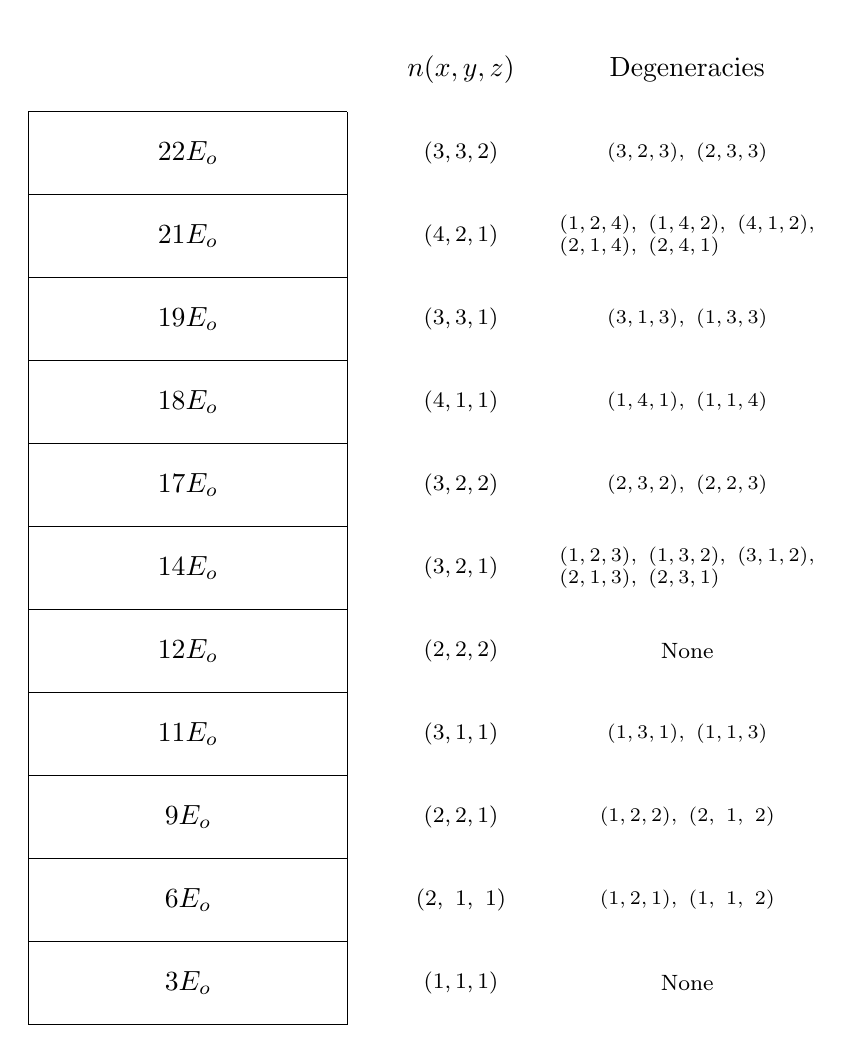
\begin{tikzpicture}[x=0.75pt,y=0.75pt,yscale=-1,xscale=1]
%uncomment if require: \path (0,538); %set diagram left start at 0, and has height of 538

%Shape: Rectangle [id:dp7431820249349796] 
\draw  [color={rgb, 255:red, 255; green, 255; blue, 255 }  ,draw opacity=1 ][fill={rgb, 255:red, 255; green, 255; blue, 255 }  ,fill opacity=1 ] (253,87) -- (362,87) -- (362,127) -- (253,127) -- cycle ;
%Shape: Rectangle [id:dp4619815785817558] 
\draw  [color={rgb, 255:red, 255; green, 255; blue, 255 }  ,draw opacity=1 ][fill={rgb, 255:red, 255; green, 255; blue, 255 }  ,fill opacity=1 ] (253,127) -- (362,127) -- (362,167) -- (253,167) -- cycle ;
%Shape: Rectangle [id:dp3359362966762425] 
\draw  [color={rgb, 255:red, 255; green, 255; blue, 255 }  ,draw opacity=1 ][fill={rgb, 255:red, 255; green, 255; blue, 255 }  ,fill opacity=1 ] (253,167) -- (362,167) -- (362,207) -- (253,207) -- cycle ;
%Shape: Rectangle [id:dp5119516390611945] 
\draw  [color={rgb, 255:red, 255; green, 255; blue, 255 }  ,draw opacity=1 ][fill={rgb, 255:red, 255; green, 255; blue, 255 }  ,fill opacity=1 ] (253,207) -- (362,207) -- (362,247) -- (253,247) -- cycle ;
%Shape: Rectangle [id:dp00577409558737596] 
\draw  [color={rgb, 255:red, 255; green, 255; blue, 255 }  ,draw opacity=1 ][fill={rgb, 255:red, 255; green, 255; blue, 255 }  ,fill opacity=1 ] (253,247) -- (362,247) -- (362,287) -- (253,287) -- cycle ;
%Shape: Rectangle [id:dp9392024809985304] 
\draw  [color={rgb, 255:red, 255; green, 255; blue, 255 }  ,draw opacity=1 ][fill={rgb, 255:red, 255; green, 255; blue, 255 }  ,fill opacity=1 ] (253,287) -- (362,287) -- (362,327) -- (253,327) -- cycle ;
%Shape: Rectangle [id:dp36507090012453736] 
\draw  [color={rgb, 255:red, 255; green, 255; blue, 255 }  ,draw opacity=1 ][fill={rgb, 255:red, 255; green, 255; blue, 255 }  ,fill opacity=1 ] (253,327) -- (362,327) -- (362,367) -- (253,367) -- cycle ;
%Shape: Rectangle [id:dp3845863388878359] 
\draw  [color={rgb, 255:red, 255; green, 255; blue, 255 }  ,draw opacity=1 ][fill={rgb, 255:red, 255; green, 255; blue, 255 }  ,fill opacity=1 ] (253,367) -- (362,367) -- (362,407) -- (253,407) -- cycle ;
%Shape: Rectangle [id:dp08289501558521084] 
\draw  [color={rgb, 255:red, 255; green, 255; blue, 255 }  ,draw opacity=1 ][fill={rgb, 255:red, 255; green, 255; blue, 255 }  ,fill opacity=1 ] (253,407) -- (362,407) -- (362,447) -- (253,447) -- cycle ;
%Shape: Rectangle [id:dp30336721777460673] 
\draw  [color={rgb, 255:red, 255; green, 255; blue, 255 }  ,draw opacity=1 ][fill={rgb, 255:red, 255; green, 255; blue, 255 }  ,fill opacity=1 ] (253,47) -- (362,47) -- (362,87) -- (253,87) -- cycle ;
%Shape: Rectangle [id:dp33732499056647836] 
\draw   (99,407) -- (253,407) -- (253,447) -- (99,447) -- cycle ;
%Shape: Rectangle [id:dp11504885678961019] 
\draw   (99,367) -- (253,367) -- (253,407) -- (99,407) -- cycle ;
%Shape: Rectangle [id:dp469041150289242] 
\draw   (99,327) -- (253,327) -- (253,367) -- (99,367) -- cycle ;
%Shape: Rectangle [id:dp5969911762901989] 
\draw   (99,287) -- (253,287) -- (253,327) -- (99,327) -- cycle ;
%Shape: Rectangle [id:dp6587152869266266] 
\draw   (99,247) -- (253,247) -- (253,287) -- (99,287) -- cycle ;
%Shape: Rectangle [id:dp7605249930787139] 
\draw   (99,207) -- (253,207) -- (253,247) -- (99,247) -- cycle ;
%Shape: Rectangle [id:dp411629440002667] 
\draw   (99,167) -- (253,167) -- (253,207) -- (99,207) -- cycle ;
%Shape: Rectangle [id:dp8033789873500379] 
\draw   (99,127) -- (253,127) -- (253,167) -- (99,167) -- cycle ;
%Shape: Rectangle [id:dp8981685875637919] 
\draw   (99,47) -- (253,47) -- (253,87) -- (99,87) -- cycle ;
%Shape: Rectangle [id:dp9045254208550346] 
\draw   (99,87) -- (253,87) -- (253,127) -- (99,127) -- cycle ;
%Shape: Rectangle [id:dp2632550671115941] 
\draw  [color={rgb, 255:red, 255; green, 255; blue, 255 }  ,draw opacity=1 ][fill={rgb, 255:red, 255; green, 255; blue, 255 }  ,fill opacity=1 ] (253,7) -- (362,7) -- (362,47) -- (253,47) -- cycle ;
%Shape: Rectangle [id:dp6780964060092816] 
\draw  [color={rgb, 255:red, 255; green, 255; blue, 255 }  ,draw opacity=1 ][fill={rgb, 255:red, 255; green, 255; blue, 255 }  ,fill opacity=1 ] (362,7) -- (471,7) -- (471,47) -- (362,47) -- cycle ;
%Shape: Rectangle [id:dp016786318374576004] 
\draw  [color={rgb, 255:red, 255; green, 255; blue, 255 }  ,draw opacity=1 ][fill={rgb, 255:red, 255; green, 255; blue, 255 }  ,fill opacity=1 ] (362,87) -- (471,87) -- (471,127) -- (362,127) -- cycle ;
%Shape: Rectangle [id:dp8106205400386881] 
\draw  [color={rgb, 255:red, 255; green, 255; blue, 255 }  ,draw opacity=1 ][fill={rgb, 255:red, 255; green, 255; blue, 255 }  ,fill opacity=1 ] (362,127) -- (471,127) -- (471,167) -- (362,167) -- cycle ;
%Shape: Rectangle [id:dp27924210424820184] 
\draw  [color={rgb, 255:red, 255; green, 255; blue, 255 }  ,draw opacity=1 ][fill={rgb, 255:red, 255; green, 255; blue, 255 }  ,fill opacity=1 ] (362,167) -- (471,167) -- (471,207) -- (362,207) -- cycle ;
%Shape: Rectangle [id:dp3175983250673733] 
\draw  [color={rgb, 255:red, 255; green, 255; blue, 255 }  ,draw opacity=1 ][fill={rgb, 255:red, 255; green, 255; blue, 255 }  ,fill opacity=1 ] (362,207) -- (471,207) -- (471,247) -- (362,247) -- cycle ;
%Shape: Rectangle [id:dp05894387939144652] 
\draw  [color={rgb, 255:red, 255; green, 255; blue, 255 }  ,draw opacity=1 ][fill={rgb, 255:red, 255; green, 255; blue, 255 }  ,fill opacity=1 ] (362,247) -- (471,247) -- (471,287) -- (362,287) -- cycle ;
%Shape: Rectangle [id:dp6291481253412834] 
\draw  [color={rgb, 255:red, 255; green, 255; blue, 255 }  ,draw opacity=1 ][fill={rgb, 255:red, 255; green, 255; blue, 255 }  ,fill opacity=1 ] (362,287) -- (471,287) -- (471,327) -- (362,327) -- cycle ;
%Shape: Rectangle [id:dp1413064646582567] 
\draw  [color={rgb, 255:red, 255; green, 255; blue, 255 }  ,draw opacity=1 ][fill={rgb, 255:red, 255; green, 255; blue, 255 }  ,fill opacity=1 ] (362,327) -- (471,327) -- (471,367) -- (362,367) -- cycle ;
%Shape: Rectangle [id:dp19360669921120954] 
\draw  [color={rgb, 255:red, 255; green, 255; blue, 255 }  ,draw opacity=1 ][fill={rgb, 255:red, 255; green, 255; blue, 255 }  ,fill opacity=1 ] (362,367) -- (471,367) -- (471,407) -- (362,407) -- cycle ;
%Shape: Rectangle [id:dp5127588021437042] 
\draw  [color={rgb, 255:red, 255; green, 255; blue, 255 }  ,draw opacity=1 ][fill={rgb, 255:red, 255; green, 255; blue, 255 }  ,fill opacity=1 ] (362,407) -- (471,407) -- (471,447) -- (362,447) -- cycle ;
%Shape: Rectangle [id:dp1536824207359908] 
\draw  [color={rgb, 255:red, 255; green, 255; blue, 255 }  ,draw opacity=1 ][fill={rgb, 255:red, 255; green, 255; blue, 255 }  ,fill opacity=1 ] (362,47) -- (471,47) -- (471,87) -- (362,87) -- cycle ;
%Shape: Rectangle [id:dp20780962546904314] 
\draw  [color={rgb, 255:red, 255; green, 255; blue, 255 }  ,draw opacity=1 ][fill={rgb, 255:red, 255; green, 255; blue, 255 }  ,fill opacity=1 ] (362,447) -- (471,447) -- (471,487) -- (362,487) -- cycle ;
%Shape: Rectangle [id:dp19273902809704002] 
\draw  [color={rgb, 255:red, 255; green, 255; blue, 255 }  ,draw opacity=1 ][fill={rgb, 255:red, 255; green, 255; blue, 255 }  ,fill opacity=1 ] (253,447) -- (362,447) -- (362,487) -- (253,487) -- cycle ;
%Shape: Rectangle [id:dp9594313478215819] 
\draw   (99,447) -- (253,447) -- (253,487) -- (99,487) -- cycle ;

% Text Node
\draw (307.5,27) node    {$n( x,y,z)$};
% Text Node
\draw (307.5,467) node  [font=\footnotesize]  {$( 1,1,1)$};
% Text Node
\draw (416.5,27) node   [align=left] {Degeneracies};
% Text Node
\draw (416.5,467) node  [font=\footnotesize] [align=left] {None};
% Text Node
\draw (307.5,427) node  [font=\footnotesize]  {$( 2,\ 1,\ 1)$};
% Text Node
\draw (307.5,387) node  [font=\footnotesize]  {$( 2,2,1)$};
% Text Node
\draw (307.5,347) node  [font=\footnotesize]  {$( 3,1,1)$};
% Text Node
\draw (307.5,307) node  [font=\footnotesize]  {$( 2,2,2)$};
% Text Node
\draw (307.5,267) node  [font=\footnotesize]  {$( 3,2,1)$};
% Text Node
\draw (307.5,227) node  [font=\footnotesize]  {$( 3,2,2)$};
% Text Node
\draw (307.5,187) node  [font=\footnotesize]  {$( 4,1,1)$};
% Text Node
\draw (307.5,147) node  [font=\footnotesize]  {$( 3,3,1)$};
% Text Node
\draw (307.5,107) node  [font=\footnotesize]  {$( 4,2,1)$};
% Text Node
\draw (307.5,67) node  [font=\footnotesize]  {$( 3,3,2)$};
% Text Node
\draw (416.5,427) node  [font=\scriptsize]  {$( 1,2,1) ,\ ( 1,\ 1,\ 2)$};
% Text Node
\draw (176,467) node    {$3E_{o}$};
% Text Node
\draw (176,427) node    {$6E_{o}$};
% Text Node
\draw (176,387) node    {$9E_{o}$};
% Text Node
\draw (176,347) node    {$11E_{o}$};
% Text Node
\draw (176,307) node    {$12E_{o}$};
% Text Node
\draw (176,267) node    {$14E_{o}$};
% Text Node
\draw (176,227) node    {$17E_{o}$};
% Text Node
\draw (176,187) node    {$18E_{o}$};
% Text Node
\draw (176,147) node    {$19E_{o}$};
% Text Node
\draw (176,107) node    {$21E_{o}$};
% Text Node
\draw (176,67) node    {$22E_{o}$};
% Text Node
\draw (416.5,387) node  [font=\scriptsize]  {$( 1,2,2) ,\ ( 2,\ 1,\ 2)$};
% Text Node
\draw (416.5,347) node  [font=\scriptsize]  {$( 1,3,1) ,\ ( 1,1,3)$};
% Text Node
\draw (416.5,307) node  [font=\footnotesize] [align=left] {None};
% Text Node
\draw (416.5,267) node  [font=\scriptsize]  {$ \begin{array}{l}
( 1,2,3) ,\ ( 1,3,2) ,\ ( 3,1,2) ,\\
( 2,1,3) ,\ ( 2,3,1)
\end{array}$};
% Text Node
\draw (416.5,227) node  [font=\scriptsize]  {$( 2,3,2) ,\ ( 2,2,3)$};
% Text Node
\draw (416.5,187) node  [font=\scriptsize]  {$( 1,4,1) ,\ ( 1,1,4)$};
% Text Node
\draw (416.5,147) node  [font=\scriptsize]  {$( 3,1,3) ,\ ( 1,3,3)$};
% Text Node
\draw (416.5,107) node  [font=\scriptsize]  {$ \begin{array}{l}
( 1,2,4) ,\ ( 1,4,2) ,\ ( 4,1,2) ,\\
( 2,1,4) ,\ ( 2,4,1)
\end{array}$};
% Text Node
\draw (416.5,67) node  [font=\scriptsize]  {$( 3,2,3) ,\ ( 2,3,3)$};


\end{tikzpicture}

      \caption{Energy Levels of $E_n(n_x,n_y,n_z)=E_o(n_x^2+n_y^2+n_z^2)$}
      \label{fig:1}
    \end{figure}

    \section*{Quantum Simple Harmonic Oscillator}

    \begin{enumerate}

      \item The principle of uncertainty explains why it is not possible for their to be no energy. The formula governing this principle is:

        $$\Delta x \Delta p \geq \dfrac{\hbar}{2}$$

        If the energy were to be zero, according to $E^2=(pc)^2+(mc^2)^2$, the momentum would be zero as well. This means:

        $$0\geq \dfrac{\hbar}{2}$$

        This is never true, as the reduced Planck constant is not negative, and thus, zero can not be greater than or equal to the value. In this manner, an energy value of 0 would violate the uncertainty principle.

      \item $E_o=\frac{1}{2}\hbar\omega_o$

        $$\hbar = \frac{h}{2\pi},\quad \omega_o=\sqrt{\frac{k}{m}}$$
        $$E_o=\frac{h}{4\pi}\sqrt{\frac{k}{m}}$$
        $$E_o=\frac{hc}{4\pi}\sqrt{\frac{k}{mc^2}}$$
        $$\frac{1240}{4\pi}\sqrt{\frac{3.5\cdot10^3}{(1.67\cdot10^{-27})(3\cdot10^8)^2}\cdot\frac{1}{1.6\cdot10^{-19}}}=.188[\si{\eV}]$$

        $$.188 << 4.5[\si{\eV}]$$

        The found energy is significantly less than the binding energy

    \end{enumerate}

\end{enumerate}

\end{document}

